\documentclass[conference,11pt]{IEEEtran}
\usepackage{hyperref}
\usepackage[numbers]{natbib}
\usepackage{mathtools}
\usepackage[pdftex]{graphicx}\bibliographystyle{IEEEtran}

\title{Relating news articles summaries\\ to stock prices}

\author{\IEEEauthorblockN{Marcelo Grossi}
    \IEEEauthorblockA{
    School of Computing\\
    Dublin City University\\
    Dublin, Ireland\\
    Email: marcelo.grossi2@mail.dcu.ie}
}

\begin{document}
\maketitle

\begin{abstract}
Stock market prediction has been a topic of great interest for researchers. Numerous attempts to ``beat the market'' have been made without been able to consistently and accurately predict the movement of stock prices.

\par
In recent years, following the increase in computational processing capabilities, researchers have been studying the relationship between news articles and stock price movement \citep{Fu2008,Schumaker2009}. Most methods are based on sentiment analysis, where the news content is classified according to its potential of moving the underlying stock's prices up (good news) or down (bad news). These methods however, do not take into account the financial instrument's context in determining the content of the news article, which greatly impairs the results of such studies. And also it is cumbersome to work with textual data in relation to numerical time series data.

\par
This work proposes a novel approach to relating textual data to stock price movements by identifying the most important terms in the daily corpus of news articles and testing for a Granger-causality between the significant terms and the price time series. This technique allows for direct analysis between aggregated news information and stock data, greatly reducing the complexity of dealing with textual information.

\par
To conclude, this study further analyses this relationship between news articles and stock price movements by using the first as regressors for predicting the latter and finds that there is a clear advantage of using all stock-related terms as covariates for predicting the target stocks price movements. Despite of the better predictions made by using the textual data, it is also found that these forecasts are not viable as a direct trading strategy.

\end{abstract}

\section{Introduction}
The relationship between news articles and stock price movements has been studied for several years \citep{gidofalvi2001,Fu2008}. The most prevalent methodology of relating news articles to stock prices is by capturing the investor sentiment \citep{Handbook} from the textual information (if it is positive, negative or neutral) and assigning a probability of whether the stock prices were likely to move upwards, downwards or stay the same. Previous researches \citep{Tetlock2007} have shown that negative sentiment predicts downward pressure on market prices, and also \citep{barber2008all} that significant news will affect the traders beliefs, what translates into an increase in trading volume.

\par
Sentiment can also be understood as the informational value of news and can be interpreted in several ways, such as via the use of financial dictionaries for analysing positive terms versus negative terms 
i.e., `profit' and `exceeds' versus `bankrupt' and `loss'; or via machine learning and natural language processing techniques to automatically generate lexicons for good and bad news sentiment \citep{Oliveira2014}, achieving excellent results compared to baseline lexicons.

\par
By using a simple na\"{\i}ve classifier, Gidófalvi \citep{gidofalvi2001} finds definite predictive power for stock price movement within a 20 minute window before and after a news article becomes publicly available. These sentiment-based analyses are very promising, and although they show high correlation with stock indicator movement it is difficult to work with textual data directly, regardless of the approach used. A general classification of sentiment (be that through dictionary/lexicon techniques or machine learning) does not take into account each stock's individual context. An extreme example would be the term `bankruptcy' which might be classified as negative in every scenario, but if a company's business is `bankruptcy attorneys' this term being on the rise might actually mean something good, as it can relate to more potential business available.

\par
This paper contributes to the area with a novel approach to the analysis of the relationship between relevant terms in a textual corpus and stock prices. By computing the relative importance of a term over time using the Term Frequency Inverse Document Frequency \citep{Ramos2003} weight, it allows for the ability to use regular tools and models for time series analysis which abstracts away the difficulties of dealing with textual data directly, as textual information is now effectively converted pragmatically into a usable time series.

\par
To evaluate this model a Granger causality test \citep{Granger1969,Granger1980} was used to assess the predictive power of the news time series over the stock price series. This test is performed between the top \(n\) most relevant terms of the day against the full set of stock prices. So the question posed is inverted; instead of asking `does this piece of news influence my stock?' we assume that news has an influence over prices, and try to find `what stocks will be influenced by the current news state?'.

\par
After selecting the term \(t\), and stock \(s\) tuples for a given day \(d\) a na\"{\i}ve ARIMAX model is tested whereby the price of day \(d+1\) is predicted and directional correctness and RMSE key performance indicators are calculated and compared.

\section{Data sources}
Online news articles from the New York Times (\url{http://www.nytimes.com/}) were used as the textual corpus of this research. Around 50,000 business-related news articles were scraped from the period between January 1\textsuperscript{st}, 2013 and October 19\textsuperscript{th}, 2014. As one of the most respected news media outlets in the world, the New York Times should provide a sufficiently good breadth of market relevant information for analysing news impact on stock prices. More specialized news providers (such as Bloomberg or Financial Times) that could potentially outperform the current data source were not considered due to their lack of impact on small investors.

\par
In order to maximize the expectation of news having an influence on stock prices, this data had to come from the same region as the news provider. Therefore, only stocks traded in the New York Stock Exchange were considered and daily price from twenty nine blue chip companies was gathered for a period that encompasses completely the news articles' database date range.

\par
A time series is a sequence of numerical data points in time successive order recorded at regular intervals. The gathered stock prices information is comprised of one daily time series of closing stock prices for each blue chip company.

\section{From text to time series}
One difficulty of working with time series and textual data is that the latter does not conform to the time series format. The data is not numerical and it is usually interpreted as one isolated event in time (usually time of publication) with no direct relationship to other textual pieces. This work brings a novel approach of converting textual data into usable time series, allowing regular time series analyses models to be applied directly.

\par
Each news article \(a\) was converted from raw unstructured textual data to a computer-friendly representation, in the form of a vector of term and related frequency \(f\), where a term \(t\) is a word \textit{n-}gram (for this experiment \textit{1} and \textit{2-}grams were used). This format is also commonly known as \textit{bag-of-words}.
\[a=[(t_1,f_1),(t_2,f_2),..,(t_n,f_n)]\]

\par
To transform the unstructured text into the \textit{bag-of-words} format a series of sequential transformations were applied. Contractions are expanded, i.e, \textit{it's} \(\to\) \textit{it is}; most common words in the English language are removed (also known as \textit{stop words}); sentences are separated (so \(n-\)grams bigger than unity can be generated only if they came from the same sentence); word tokenization (transform sentence \(s\) in a collection of words \(W_s\)) is used; part-of-speech tagging (or \textit{POST}) was performed in each sentence (disambiguate each word's grammatical function, i.e., adjective, subject, verb, etc.); word lemmatization (use \textit{POST} extracted in the previous step to calculate the word's lemma, i.e., \textit{saw, verb} \(\to\) \textit{see} or \textit{saw, subject} \(\to\) \textit{saw}); and finally generation of \(n-\)grams -- i.e., given that \(W_{s_1}=[w_1,w_2,..,w_n]\) is a set of words from sentence one, the \textit{2-}grams collection would be of the form \([w_1 w_2,w_2 w_3,..,w_{n-1} w_n]\).

\par
Each news article (converted to \textit{bag-of-words}) \(a \in A\) was grouped by the date \(d\) it was published, and a daily summary was produced whereby a score was assigned to each \(n-\)gram following the Term Frequency Inverse Document Frequency algorithm (\textit{tfidf}).

\[TS_t=({tfidf_{t_d}}, \forall d \in D)\]

This score is calculated by multiplying the \(n-\)gram frequency (number of times \(n-\)gram \(t\) appears in all of \(A_d\) over the total number of \(n-\)grams in \(A_d\)) by the logarithm of the inverse of the document frequency (total number of articles in the day \(\vert A_d \vert\) over the number of articles \(\vert A_t \vert\) that \(n-\)gram \(t\) appears in). Another way of understanding the \(tfidf_{t_d}\) is that it expresses the relative importance of \(n-\)gram \(t\) over the course of day \(d\). So even if a term (or \(n-\)gram) appears in most documents with very high frequency (high \(tf\)), it will get heavily penalized by the \(idf\), where \(0 \leq tfidf_t\). Although the score is unbounded in its upper limits, it is expected that in an unbiased big collection of articles, this value stays close to zero (this is due to the normalization of the \(tf\) whereby the individual frequencies are divided by the total frequency of the day).
From the daily summaries obtained through \(tfidf\) it becomes straight forward to calculate a time series \(TS\) for any \(n-\)gram \(t\) given a set of all days \(D\).

\section{Selecting terms and stocks}
One of the objectives of this research is to find if there is a relationship between the daily stock prices and the time series produced from the textual corpus. A brute force approach will not be attempted, as there are roughly 30,000 different \(n-\)grams each day and those in the lower end of the \(TFIDF\) weighing scheme are either too frequent to be of any use, or too infrequent so as to not have enough data to be relevant. For this study, an arbitrary amount of \(100\) \(n-\)grams with the best score are selected from each day's summary, and a time series is extracted for each one. This set will henceforth be known as \(T_d\).

\par
The set of stock price data \(S_d\), as a dependent variable, is a slice from the complete stock price information from January 1\textsuperscript{st}, 2013 to \(d\); where \(d\) is the day being evaluated for the independent variables in \(T_d\). Interpolation is performed in \(S_d\) at this point, to make sure all news data points are captured and potential relevant information published on weekends or holidays is properly modelled.

\par
In order to produce the final term \(t_d \in T_d\), stock \(s_d \in S_d\) tuples a test must be performed to validate wether or not \(t_d\) has any prediction power over \(s_d\). With that same objective, Granger \citep{Granger1969,Granger1980} proposed a \textit{predictive causality} statistical test to determine if a time series is useful in forecasting another. This \textit{Granger-causality test}, or simply \textit{Granger test} is based on two fundamental principles according to Eichler \citep{eichler2012}:

\begin{enumerate}
\item ``the effect does not precede its cause in time'';
\item ``the cause has unique information about the series being caused that is not available otherwise'';
\end{enumerate}

\par
Following from these principles, the \textit{Granger test} model can then be formulated by letting \(y\) and \(x\) be two stationary time series, where the null hypothesis is that \(x\) does not \textit{Granger-cause} \(y\), if the \textit{F-test} (or \textit{Wald test}) between a univariate auto-regression of \(y\) (equation~\ref{eq:1}) and a multivariate auto-regression of both \(y\) and \(x\) (equation~\ref{eq:2}) fails to find any explanatory power after the exogenous variable \(x\) is added to the model.

\begin{equation}
\label{eq:1}
y_t=\beta_0 + \beta_1 y_{t-1} + \beta_2 y_{t-2} + .. + \beta_n y_{t-n} + \varepsilon_t
\end{equation}
\begin{equation}
\label{eq:2}
y_t=\beta_0 + \beta_1 y_{t-1} + .. + \beta_n y_{t-n} + 
\alpha_1 x_{t-1} + .. + \alpha_n x_{t-n}
+ \varepsilon_t
\end{equation}

\par
It is not uncommon to find a bi-directional causality relationship between the variables when \textit{Granger-testing}, therefore both directions are tested and if no causality is found, or the causality is found in both directions the tuple is disregarded. Furhter information on the actual methodology used for testing \textit{Granger-causality} in this study can be found in \citep{Toda1995}, or excellently summarized in \citep{Giles2011}.

\par
The resulting tuples \((t_d, s_d)\) where \(t_d \xrightarrow[causes]{Granger} s_d\) (and \(t_d \not\xleftarrow[causes]{Granger} s_d\)) can now be used to test the effectiveness of the predicting power of \(t_d\) over \(s_d\). A sample of such relationship can be seen in figure~\ref{fig:term_stocks} where terms related to stocks `KO' (\textit{Coca-Cola Co.}) and `PFE' (\textit{Pfizer Inc.}) are shown for \(d=14/08/2014\) (this day was chosen to allow a \(9:1\) split of the dataset, saving \(10\%\) for the tests).

\begin{figure}[!htbp]
\centering
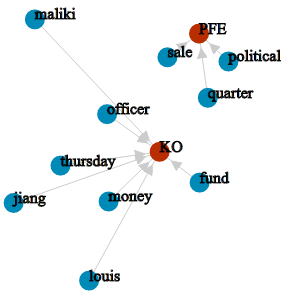
\includegraphics[width=2.5in]{force_20140814_small}
\caption{Directed graph sample of \textit{Granger-causing} terms (\textit{blue}) and stock symbols (\textit{brown})}
\label{fig:term_stocks}
\end{figure}

\section{Predicting price movements}
To validate the predicting potential of the generated term time series, a model is chosen to fit the data and forecast out-of-sample prices for the stocks using the term time series as regressors. These results are then compared to the same model without any regressors to assess whether or not the term time series has an influence on stock prices (if prediction made with terms is better than without the terms it becomes patent it's influence). To finalize, a test to measure the ability of the predictions to be used as an investment strategy is proposed in order to evaluate the usefulness of this model in real world scenarios.

\par
Widely used in time series analysis, and first introduced by Box and Jenkins in 1976 (recently reviewed in \citep{box2008time}) the \textit{autoregressive integrated moving average with exogenous variable} (\textit{ARIMAX}) model is fit to each term, stock tuples, where the stock price series is the target function and the term series functions as a predictor (or exogenous variable). The tests are performed using each term series as an exogenous variable individually, then all term series related to a stock are used as exogenous variables to fit the same model. A final model is fit to the stock prices without any predictors, to serve as the baseline for further comparisons. These models are henceforth referred to as the individual (\(Ind\)), aggregated (\(Agg\)) and no-exogenous models (\(NoEx\)).

\par
The \textit{ARIMAX} model, which is an integrated variation of the \textit{ARMA} model with exogenous variables, is fit for modelling auto-correlated data with or without seasonality components (in this study only the non-seasonal variety is used), where the integrated part is a  shorthand for differencing the series before calculating the coefficients to ensure stationary. The introduction of exogenous variables in the model involves the addition of the covariate \(x_t\) to the right hand side of the \textit{ARMA} formula. Equations~\ref{eq:4} and \ref{eq:5} show the \textit{ARMA(p,q)} and \textit{ARMAX(p,q)} models respectively, where \(z_t\) is a white noise process.

\begin{equation}
\label{eq:4}
y_t=\phi_1 y_{t-1} + .. + \phi_p y_{t-p} - 
\theta_1 z_{t-1} - .. - \theta_q z_{t-q} +
z_t
\end{equation}

\begin{equation}
\label{eq:5}
y_t=\beta x_t + \phi_1 y_{t-1} + .. + \phi_p y_{t-p} - 
\theta_1 z_{t-1} - .. - \theta_q z_{t-q} +
z_t
\end{equation}

\par
To asses the quality of time series forecasts, it is usual to calculate the root mean squared errors (or \textit{RMSE}) and compare it against other RMSE's produced by different models on the same dataset, the model with lowest RMSE performs best. As the objective in this study is to compare the forecast quality across different time series (with potentially different price intervals), a scaling function is applied to the stock price series before calculating the RMSE (a scaled series can be understood in this context as a time series whose values lie within the \([0,1]\) interval, and equation~\ref{eq:3} shows the scaling function \(SCALE_{s}\) for stock series \(s\)).

\begin{equation}
\label{eq:3}
SCALE_{s}=\frac{s-\min s}{\max \{s-\min s\}}
\end{equation}

\par
Lastly, a tradeability test is performed to verify if this technique can be used directly as a viable investment strategy. Several approaches can be used to assess tradeability, the most usual being the construction of a full trading strategy surrounding the signals produced by the model. This can be very cumbersome and prone to masking the real performance of the underlying signal generating model, by use of clever investment strategies one can produce profits that are completely unrelated to the model being tested.

\par
To avoid this pitfall, a simple directional correctness ratio measure is introduced where if for day \(d\) the predictions (individual, aggregated and no-exogenous) are able to correctly forecast the direction in which the prices have moved the following day \(d+1\), it is considered correct. If the correctness rate is found to be better than random (far from \(50\%\)), it is considered a viable strategy. Note that even if the correctness rate is far below \(50\%\) it can still be considered viable, as all an investor has to do is invert the signal.

\par
These tests are computed for all days of the test dataset (namely, the interval between 14/08/2014 and 20/09/2014).

\section{Results}
<TODO:MORE CONCLUSIONS CAN BE DRAWN FROM THIS?>
The tuples generated for \textit{Granger-causing} terms and stocks were quite interesting. The term \textit{`loan'} was matched with stock prices from \textit{Alcoa}, \textit{Intel}, \textit{Merck \& Co.}, and \textit{Microsoft} indicating a predictive relationship between the historic relative importance of this term in the New York Times media coverage news corpus and the aforementioned companies' stock prices, as traded in the New York Stock Exchange.

\par
The philosophy of why this term is related to these particular stocks is outside the scope of this research but other more peculiar terms were also matched with several stocks. Terms such as `billion', `million', `could', `year' and `thursday'  were inexplicably found to have a \textit{Granger-causal} relationship with many blue chip stock prices. Given the common and widespread usage of these terms, they may have biased the \textit{TFIDF} score making the interpretation of their relative importance into a proxy of some other generating factor - perhaps the volume of news produced? Or something else entirely.

\par
The individual and no-exogenous models performed similarly, with a slight edge to the individual models. The aggregated models performed best in both measures (\(RMSE\) and \(directional correctness\)). Although there is a definitive improvement from the no-exogenous models to their exogenous counterparts, no model has showed significant tradeability potential.

\par
The \textit{ARIMAX} model turned out to be a poor predictor of the stock series, failing to fit the data exceptionally well. It would be interesting to analyse the same dataset with a collection of more advanced time series models. Such exploration work will not be performed here as this model was merely an example of what can be done with the generated term time series, and also to compare its performance against that of the no-exogenous model.

\par
The directional correctness ratio indicator showed a variation between \(35\%\) and \(63\%\) correctness, with an average of \(49.9\%\) and variance of \(0.43\%\). This result, coupled with a  t-test (with \(5\%\) significance) indicates that the predictions made by the model are no better than random and that using this model with the term time series is not directly translatable into winning trading strategies. Figure~\ref{fig:dir_corr_hist} plots the directional correctness binned frequencies and it shows quite clearly the aggregate models' superiority if compared to the individual and no-exogenous models.

\begin{figure}[!htbp]
\centering
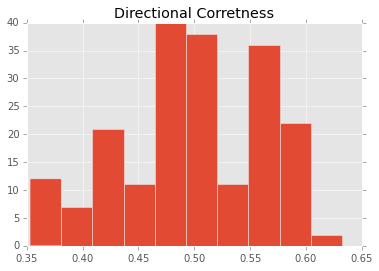
\includegraphics[width=3.5in]{dir_corr_hist}
\caption{Directional correctness ratio of forecasts binned frequencies}
\label{fig:dir_corr_hist}
\end{figure}

\par
The best directional correctness results were for the stock symbols \textit{KO} (Coca-Cola Co., using exogenous series from term \textit{``money''}) and \textit{PFE} (Pfizer Inc., using exogenous series from term \textit{``quarter''}) with \(35\%\) and \(63\%\) correctness respectively. Inverting the directional predictions of Coca-Cola Co. would yield a correctness rate of \(65\%\), becoming slightly better than Pfizer's.

\par
The root mean square error measure allows for a direct comparison between the individual, aggregated and no-exogenous models. The results in this area corroborate the directional correctness results, showing that in general, the aggregated model fairs better than the individual and no-exogenous models. This clearly indicates that using all available information is more advantageous than modelling the terms individually and also than not using the term time series at all. The descriptive statistics of this indicator can seen in table~\ref{tab:1} and figure~\ref{fig:rmse_line}.

\begin{table}
\caption{Root mean square error}
\label{tab:1}
\begin{tabular}{ r c c c c c }
             & Obs   & Min   & Max   & \(\mu\) & \(\sigma^2\) \\
All          & 219   & 0.035 & 0.584 & 0.148   & 0.007 \\ 
Individual   & 165   & 0.043 & 0.583 & 0.148   & 0.007 \\
Aggregated   & 26    & 0.056 & 0.322 & 0.141   & 0.006 \\
No-exogenous & 28    & 0.035 & 0.584 & 0.153   & 0.012 \\
\end{tabular}
\end{table}

\begin{figure}[!htbp]
\centering
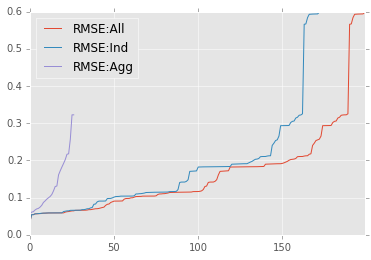
\includegraphics[width=2.5in]{rmse_line}
\caption{Root mean square error for individual, aggregated and no-exogenous models}
\label{fig:rmse_line}
\end{figure}

\par
For more detailed information, the complete research, code and results can be found at \url{https://github.com/magrossi/news_n_stocks}.

\section{Conclusion}
Using public and free data sources, a different approach of relating textual data and stock price movements is introduced by generating term time series data pragmatically from \(TFIDF\) scores. This novel technique allows for a fully contextualized analysis of  textual and stock data, and eliminates the cumbersomeness of dealing with textual data directly.

\par
A validation model for the ability of the generated term time series to forecast stock price movements was tested and although it did not show direct tradeability capabilities, it clearly indicated that modelling stock prices using all related term time series is more advantageous and should encourage investors to use textual information in their predicting models to increase the quality of their output trading signals.

\par
Some caveats are important to be mentioned. Using a larger dataset, that spanned multiple years and sourced from different providers, would help offset potential editorial biases and increase variance. Also, if both the time and date of publishing were available for each news article, an equivalent intra-day research could show different insights into news and stock relationship.

\par
Future research may include repeating this same experiments using different textual filtering options, such as capturing only nouns or named entities from the textual corpus to avoid some of the more peculiar results founds here. Another avenue of study can be to compare the effectiveness of different news sources; or build a directed term to stock graph and procure unknown relationships between stocks of different sectors or with weak intuitive relationships. Experimenting with different time series models such as transfer models, VAR, VECM, and others, then compare results can also be a very interesting research path.

\bibliography{IEEEabrv,practicum_marcelo_grossi}

\end{document}